%analysis body
%Created MS 05-11

\section{Analysis}\label{analysis}

\subsection{$^{85}$Rb and $^{87}$Rb Spin Analysis}

By measuring the resonant RF frequencies used to induce the coupling of $m_F$ states, we can calculate the $g$-factors for $^{85}$Rb and $^{87}$Rb.  In in Section \ref{linewidth}, we found the resonant frequencies to be $161.7$ kHz for $^{85}$Rb and $243.0$ kHz for $6{87}$Rb.  (values for B, n, I?) Using Equation \ref{BLAH} we calculate $g_F$ for $^{85}$Rb to be $0.30\pm BLAH$ and $g_F$ for $^{87}$Rb to be $0.46\pm BLAH$.  Both calculations are in good agreement with the theoretical values of $1/3$ and $1/2$ respectively. 

Using Equation \ref{eq:BLAH} and our calculated values for $g_F$, we can calculate the nuclear spins of both $^{85}$Rb and $^{87}$Rb in the $^{2}S_{1/2}$ atomic states.  Doing so, we calculate the nuclear spins to be $2.8 \pm BLAH$ and $1.7 \pm BLAH$ respectively.  These calculations are in good agreement with the theoretical values of $5/2$ and $3/2$.

Error Analysis

\subsection{Time Evolution Analysis}

\subsubsection{Determination of $T_{2}$ Relaxation Time}

By measuring the natural linewidth of $^{85}$Rb , we can calculate the $T_2$ relaxation time.  In Section \ref{linewidthmeas}, we found that the natural linewidth of $^{85}$Rb was $370$ kHz.  Using Equation \ref{eq:T2}, we calculate $T2$ to be 


\subsubsection{Determination of the $T_{1}$ Relaxation Time}

\begin{figure}[htbp]
\begin{center}
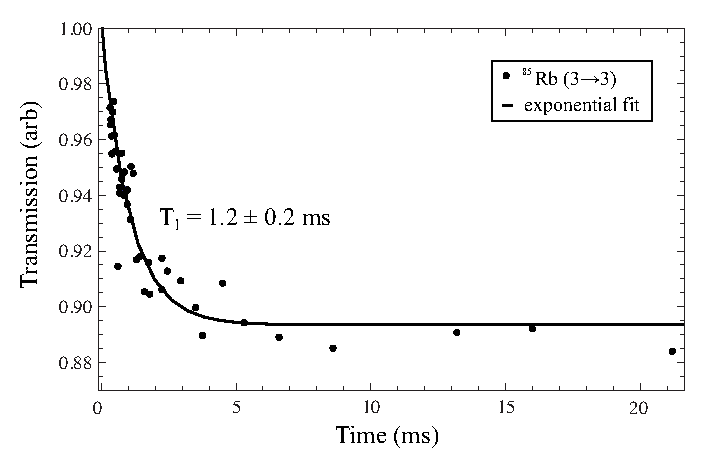
\includegraphics[height=70mm]{./figures/T1.eps}
\caption{\small{}}
\label{fig:}
\end{center}
\end{figure}

\subsubsection{Determination of the Optical Pumping Time}

\subsection{Spin Exchange Analysis}

\subsubsection{Determination of $T_{\mathrm{SE}}$}

\subsubsection{Determination of $\sigma_{\mathrm{SE}}$}